%%%%%%%%%%%%%%%%%%%%%%%%%
\section{مسئله‌های ان‌پی کامل}
%%%%%%%%%%%%%%%%%%%%%%%%%

\begin{frame}{مسئله‌های ان‌پی کامل}
\begin{itemize}\itmsep{2mm}
\item[-]
بسیاری از الگوریتم‌هایی که در مبحث طراحی الگوریتم‌ها بررسی کردیم، الگوریتم‌های زمان
\fn{1}{polynomial-time algorithm}
چند جمله‌ای بودند بدین معنی که به ازای ورودی با اندازهٔ
\m{n}
، زمان اجرای آنها در بدترین حالت به ازای ثابت
\m{k}
برابر است با
\m{O(n^k)} .
\item[-]
اما همهٔ مسئله‌ها در زمان چند جمله‌ای قابل محاسبه نیستند.
\item[-]
برخی از مسئله‌ها مانند مسئلهٔ توقف
\fn{2}{halting problem}
(توقف‌پذیری یک برنامه بر روی یک ورودی)
یا مسئلهٔ دهم هیلبرت (حل‌پذیری معادلات سیاله
\fn{3}{diophantine equations}
)،
 نه تنها در زمان چند جمله‌ای قابل محاسبه نیستند، بلکه توسط هیچ الگوریتمی قابل محاسبه نیستند.
\item[-]
معمولاً به مسائلی که در زمان چند جمله‌ای قابل حل هستند، مسائل آسان و به مسائلی که در زمان چند جمله‌ای قابل محاسبه نیستند، مسائل سخت
\fn{4}{hard problem}
یا غیر قابل کنترل
\fn{5}{intractable}
می‌گوییم.
\end{itemize}
\end{frame}


\begin{frame}{مسئله‌های ان‌پی کامل}
\begin{itemize}\itemr
\item[-]
در این قسمت می‌خواهیم دسته‌ای از مسائل را معرفی کنیم که به آنها مسائل ان‌پی کامل
\fn{1}{NP-complete problems}
می‌گوییم.
پیچیدگی محاسباتی مسائل ان‌پی کامل نامعلوم است. هیچ الگوریتم چند جمله‌ای برای این دسته از مسائل تاکنون پیدا نشده است و کسی نتوانسته اثبات کند که هیچ الگوریتم چند جمله‌ای برای آنها وجود ندارد.
\item[-]
مسئلهٔ پی در برابر ان‌پی
\fn{2}{P vs. NP}
یکی مسائل حل نشدهٔ مهم در علوم کامپیوتر است که در مورد آن صحبت خواهیم کرد.
\item[-]
برخی از مسائل محاسباتی بسیار شبیه یکدیگر هستند و با وجود شباهت ظاهری‌شان برای یکی از آنها الگوریتم چند جمله‌ای وجود دارد و دیگری در دستهٔ مسائل ان‌پی کامل است.
در اینجا به برخی از این مسائل اشاره می‌کنیم.
\end{itemize}
\end{frame}


\begin{frame}{مسئله‌های ان‌پی کامل}
\begin{itemize}\itemr
\item[-]
مسئله کوتاهترین مسیر در مقابل مسئله بلندترین مسیر : با این که این دو مسئله بسیار شبیه یکدیگرند، اما برای مسئله کوتاهترین مسیر در گراف یک الگوریتم چند جمله‌ای وجود دارد که در زمان
\m{O(|V||E|)}
اجرا می‌شود، اما مسئله بلندترین مسیر یک مسئلهٔ ان‌پی کامل است.
\item[-]
مسئلهٔ دور اویلری و دور همیلتونی : دور اویلری
\fn{1}{Eulerian cycle}
در یک گراف دوری است که از هر یال دقیقا یک بار عبور می‌کند. این دور می‌تواند از هر رأس چندبار عبور کند. این مسئله در زمان
\m{O(|E|)}
برای گراف
\m{G(V,E)}
قابل حل است.  دور همیلتونی
\fn{1}{Hamiltonian cycle}
 دوری است که از هر رأس دقیقا یک‌بار عبور می‌کند. این مسئله یک مسئله ان‌پی کامل است.
\end{itemize}
\end{frame}


\begin{frame}{مسئله‌های ان‌پی کامل}
\begin{itemize}\itemr
\item[-]
مسئلهٔ صدق‌پذیری ۲ تایی و صدق پذیری ۳ تایی : عبارات منطقی شامل متغیرهای منطقی هستند که مقدار آنها می‌تواند صفر یا یک باشد. این متغیرها به عنوان عملوند با تعدادی عملگر منطقی عبارات منطقی را می‌سازند. عملگرهای منطقی شامل عملگر عطف
\fn{1}{conjunction}
\m{(\wedge)}
، عملگر فصل
\fn{2}{disjunction}
\m{(\vee)}
و عملگر نقیض
\fn{3}{negation}
\m{(\sim)}
می‌شوند.
\item[-]
یک عبارت صدق پذیر
\fn{4}{safisfiable}
است اگر با انتساب مقادیر صفر و یک به متغیرهای عبارت، مقدار عبارت برابر با ۱ شود. یک عبارت به صورت فرم نرمال عطفی k تایی است اگر آن عبارت از عطف چندین عبارت تشکیل شده باشد که هر یک از آن عبارات از فصل k متغیر یا نقیض متغیر تشکیل شده باشند.
\item[-]
مسئلهٔ صدق پذیری ۲ تایی در واقع تعیین صدق پذیری یک عبارت به صورت فرم نرمال ۲ تایی است. گرچه برای مسئلهٔ صدق پذیری ۲ تایی الگوریتم چندجمله‌ای وجود دارد، اما صدق‌پذیری ۳ تایی ان‌پی کامل است.
\end{itemize}
\end{frame}


\begin{frame}{مسئله‌های ان‌پی کامل}
\begin{itemize}\itemr
\item[-]
سه دسته از مسائل مهم محاسباتی را در اینجا به صورت غیر رسمی تعریف می‌کنیم : مسائل پی، مسائل ان‌پی و مسائل ان‌پی کامل.
\item[-]
کلاس پی
\fn{1}{class P}
شامل مسائلی است که در زمان چند جمله‌ای 
\fn{2}{polynomial time}
قابل حل هستند. این دسته از مسائل در زمان
\m{O(n^k)}
به ازای ثابت k قابل حل هستند، جایی که n اندازهٔ ورودی مسئله است. بسیاری از مسائلی که تا اینجا مورد بررسی قرار دادیم در کلاس پی قرار دارند.
\item[-]
کلاس ان‌پی
\fn{3}{class NP}
شامل مسائلی است که در زمان چند جمله‌ای قابل تصدیق
\fn{4}{verifiable}
هستند، بدین معنی که اگر یک مقدار به عنوان جواب داده شود، در زمان چند جمله‌ای می‌توان بررسی کرد که آیا مقدار داده شده یک جواب درست است یا خیر. برای مثال اگر برای یک گراف یک دور داده شود، می‌توان در زمان چند جمله‌ای بررسی کرد آیا دور داده شده همیلتونی است یا خیر.
\end{itemize}
\end{frame}


\begin{frame}{مسئله‌های ان‌پی کامل}
\begin{itemize}\itemr
\item[-]
هر مسئله در کلاس پی به کلاس ان‌پی نیز متعلق دارد، زیرا اگر یک مسئله در زمان چند جمله‌ای قابل حل باشد، در زمان چند جمله تصدیق‌پذیر نیز هست. بنابراین می‌توان بگوییم
\m{P \subseteq NP}.
\item[-]
مسئله مشهور پی در مقابل ان‌پی
\fn{1}{P vs NP}
می‌پرسد آیا کلاس پی و ان‌پی برابرند یا خیر. به عبارت دیگر آیا مسائلی که در زمان چند جمله‌ای قابل تصدیق هستند، در زمان چند جمله‌ای قابل حل هستند یا خیر؟
\item[-]
یک مسئله به دستهٔ مسائل ان‌پی کامل
 \fn{2}{NP-complete}
تعلق دارد اگر عضو کلاس ان‌پی باشد و همچنین به سختی همهٔ مسائل ان‌پی است. 
%در آینده درجه سختی را به طور رسمی تعریف می‌کنیم. 
به عبارت دیگر اگر هر یک از مسائل ان‌پی کامل در زمان چند‌جمله‌ای حل شوند، آنگاه همهٔ مسائل ان‌پی در زمان چند‌جمله‌ای حل می‌شوند.
\end{itemize}
\end{frame}


\begin{frame}{مسئله‌های ان‌پی کامل}
\begin{itemize}\itemr
\item[-]
بسیاری از دانشمندان علوم کامپیوتر بر این باورند که مسائل ان‌پی هیچ‌گاه در زمان چند‌جمله‌ای حل نخواهند شد.
\item[-]
به عنوان یک طراح الگوریتم، اگر بتوانید ثابت کنید که یک مسئله ان‌پی کامل است، به احتمال زیاد به راحتی برای آن الگوریتم چندجمله‌ای پیدا نخواهید کرد، بنابراین بهتر است تمرکز خود را بر روی پیدا کردن یک الگوریتم تقریبی خوب بگذارید یا مسئله را برای حالت‌های خاص حل کنید.
\item[-]
اگر ثابت کنید یک مسئله ان‌پی کامل است، در واقع می‌توانید سختی آن مسئله را نشان دهید و نشان دهید جستجو برای یک الگوریتم چندجمله‌ای به احتمال بسیار زیاد بی ثمر خواهد بود.
\end{itemize}
\end{frame}


\begin{frame}{مسئله‌های ان‌پی کامل}
\begin{itemize}\itemr
\item[-]
بسیاری از مسئله‌ها، مسائل بهینه سازی
\fn{1}{optimization problem}
هستند و هدف از حل این مسائل یافتن مقداری است که از جواب‌های دیگر بهتر (کوچکتر، بزرگتر، ...) است. برای مثال مسئله کوتاهترین مسیر، یک مسئلهٔ بهینه سازی است، زیرا در میان همهٔ مسیرهای ممکن، هدف پیدا کردن مسیری است که در طول آن از همه کمتر است.
\item[-]
مسائل ان‌پی کامل مسائل بهینه سازی نیستند، بلکه مسائل تصمیم‌گیری
\fn{2}{decision problem}
هستند. در این‌گونه مسائل جواب بله و خیر است.
\item[-]
با این حال مسائل بهینه‌سازی قابل تبدیل به مسائل تصمیم‌گیری هستند. برای مثال به ازای یک گراف و دو رأس u و v و مقدار k می‌توانیم بپرسیم آیا مسیری با طول k از u به v وجود دارد یا خیر.
\item[-]
پس اگر نشان دهیم یک مسئلهٔ تصمیم‌گیری ان‌پی کامل است، مسئلهٔ بهینه‌سازی متناظر با آن نیز ان‌پی کامل خواهد بود.
\end{itemize}
\end{frame}


\begin{frame}{مسئله‌های ان‌پی کامل}
\begin{itemize}\itemr
\item[-]
حال می‌خواهیم نشان دهیم که یک مسئله از مسئلهٔ دیگر سخت‌تر نیست.
\item[-]
معمولاً یک مسئله در حالت کلی توسط تعدادی پارامتر بیان می‌شود. وقتی پارامترهای یک مسئله را مقداردهی می‌کنیم در واقع یک نمونه
\fn{1}{intance}
از مسئله را به دست آورده‌ایم.
\item[-]
برای مثال مسئلهٔ کوتاهترین مسیر می‌پرسد به ازای یک گراف دلخواه و دو رأس u و v چگونه کوتاهترین مسیر را در حالت کلی پیدا کنیم. یک نمونه از مسئله درواقع یک گراف معین و دو رأس ورودی و خروجی معین است.
\end{itemize}
\end{frame}


\begin{frame}{مسئله‌های ان‌پی کامل}
\begin{itemize}\itemr
\item[-]
مسئلهٔ تصمیم‌گیری A را در نظر بگیرید که می‌خواهید آن را در زمان چندجمله‌ای حل کنید.
\item[-]
فرض کنید می‌دانید چگونه مسئله B را در زمان چند‌جمله‌ای حل کنید.
\item[-]
همچنین فرض کنید می‌دانید چگونه هر نمونه
\m{\alpha}
از مسئله A رابه نمونهٔ
\m{\beta}
از مسئلهٔ B تبدیل کنید به طوری‌که :\\
۱. تبدیل نمونه
\m{\alpha}
به نمونه
\m{\beta}
در زمان چند‌جمله‌ای انجام شود.\\
۲. جواب نمونه مسئله تصمیم‌گیری
\m{\alpha}
بله باشد اگر و تنها اگر جواب نمونه مسئلهٔ تصمیم‌گیری
\m{\beta}
بله باشد.
\item[-]
چنین روندی برای تبدیل مسئله‌های تصمیم‌گیری به یکدیگر را الگوریتم کاهش در زمان چندجمله‌ای
\fn{1}{polynominal time reduction algorithm}
می‌نامیم.
\item[-]
اگر B در زمان چندجمله‌ای قابل حل باشد و A در زمان چندجمله‌ای قابل کاهش به B باشد، آنگاه برای حل مسئلهٔ A در زمان چندجمله‌ای کافی است آن را در زمان چندجمله‌ای به B کاهش دهیم و سپس B را در زمان چندجمله‌ای حل کنیم.
\end{itemize}
\end{frame}


\begin{frame}{مسئله‌های ان‌پی کامل}
\begin{itemize}\itemr
\item[-]
الگوریتم کاهش در زمان چندجمله‌ای در واقع روشی برای حل مسئله A در زمان چند‌جمله‌ای است.\\
۱. به ازای نمونه
\m{\alpha}
از مسئله A ، از الگوریتم کاهش در زمان چندجمله‌ای برای تبدیل آن به نمونه
\m{\beta}
از مسئله B استفاده می‌کنیم.\\
۲. مسئله تصمیم‌گیری B را برای نمونه
\m{\beta}
در زمان چندجمله‌ای حل می‌کنیم.\\
۳. جواب نمونه
\m{\beta}
را به عنوان جواب نمونه
\m{\alpha}
در نظر می‌گیریم.
\end{itemize}
\end{frame}


\begin{frame}{مسئله‌های ان‌پی کامل}
\begin{itemize}\itemr
\item[-]
شکل زیر الگوریتم کاهش برای حل یک مسئله را نشان می‌دهد.
\begin{figure}
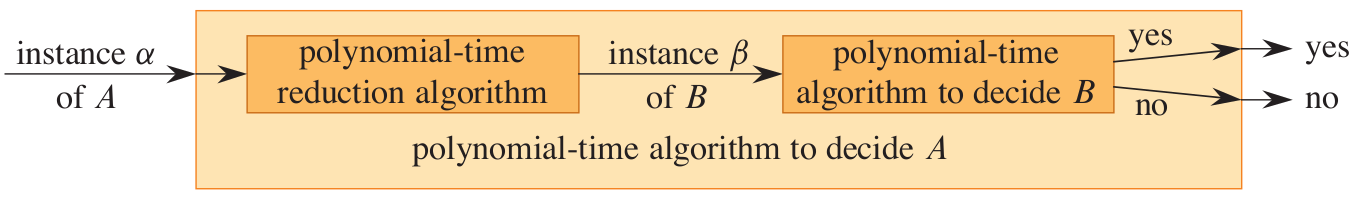
\includegraphics[width=0.9\textwidth]{figs/chap08/1046-reduction}
\end{figure}
\end{itemize}
\end{frame}


\begin{frame}{مسئله‌های ان‌پی کامل}
\begin{itemize}\itemr
\item[-]
پس با استفاده از روش کاهش برای حل مسئله A از الگوریتم چندجمله‌ای مسئله B استفاده می‌کنیم.
%\item[-]
%پس آسان بودن مسئلهٔ B روشی آسان برای حل مسئله A ارائه می‌دهد.
\item[-]
از همین ایده استفاده می‌کنیم برای اینکه نشان دهیم یک مسئله به سختی یک مسئلهٔ دیگر است.
\end{itemize}
\end{frame}


\begin{frame}{مسئله‌های ان‌پی کامل}
\begin{itemize}\itemr
\item[-]
فرض کنید ثابت شده‌است که برای مسئله A الگوریتم چندجمله‌ای وجود ندارد. حال فرض کنید یک الگوریتم کاهش در زمان چندجمله‌ای برای تبدیل یک نمونه از مسئله A به یک نمونه از مسئله B وجود دارد. می‌توانیم با استفاده از برهان خلف نشان دهیم که هیچ الگوریتم چندجمله‌ای برای B وجود ندارد.
\item[-]
برای اثبات این قضیه فرض کنید برای B یک الگوریتم چندجمله‌ای وجود داشته باشد، در آن صورت می‌توانستیم با استفاده از کاهش، یک الگوریتم چندجمله‌ای برای A پیدا کنیم، اما می‌دانیم ثابت شده است که الگوریتم چندجمله‌ای برای A وجود ندارد. پس به تناقض می‌رسیم و در نتیجه فرض اولیه نادرست بوده و الگوریتم چندجمله‌ای برای ‌B وجود ندارد.
\end{itemize}
\end{frame}

\begin{frame}{مسئله‌های ان‌پی کامل}
\begin{itemize}\itemr
\item[-]
برای اینکه نشان دهیم B ان‌پی کامل است از همین روند استفاده می‌کنیم. اگرچه نمی‌توانیم به طور قطعی بگوییم که هیچ الگوریتم چندجمله‌ای برای A وجود ندارد، اما می‌توانیم اثبات کنیم B ان‌پی کامل است با فرض اینکه A ان‌پی کامل است.
پس برای اثبات ان‌پی کامل بودن یک مسئله باید یکی از مسائل ان‌پی‌کامل را در زمان چندجمله‌ای به آن مسئله کاهش دهیم.
می‌گوییم مسئلهٔ B به سختی مسئلهٔ A است.
\item[-]
اولین مسئله‌ای که ان‌پی کامل بودن آن اثبات شده است، مسئلهٔ صدق پذیری است.
برای اثبات اولین مسئله اثبات شد که همهٔ مسائل ان‌پی در زمان چندجمله‌ای قابل کاهش به مسئلهٔ صدق‌پذیری هستند. بنابراین اگر مسئلهٔ صدق‌پذیری در زمان چندجمله‌ای حل شود، همهٔ مسائل ان‌پی در زمان چندجمله‌ای حل خواهند شد. به عبارت دیگر مسئلهٔ صدق‌پذیری به سختی همهٔ مسائل ان‌پی است.
\item[-]
در واقع هر یک از مسائل ان‌پی‌کامل به سختی همهٔ مسائل ان‌پی است، زیرا حل یکی از آنها در زمان چندجمله‌ای منجر به حل همهٔ مسائل ان‌پی می‌شود.
\end{itemize}
\end{frame}